\documentclass[a4paper,10pt]{article}
\usepackage[a5paper, margin=10mm, onecolumn]{geometry}

\usepackage{tfrupee}
\setlength{\headheight}{1cm}
\setlength{\headsep}{0mm}

\usepackage{gvv-book}

\usepackage{cite}
\usepackage{amsmath,amssymb,amsfonts,amsthm}
\usepackage{gvv}
\usepackage{algorithmic}
\usepackage{graphicx}
\usepackage{textcomp}
\usepackage{xcolor}
\usepackage{txfonts}
\usepackage{listings}
\usepackage{enumitem}
\usepackage{mathtools}
\usepackage{gensymb}
\usepackage{comment}
\usepackage[breaklinks=true]{hyperref}
\usepackage{tkz-euclide} 
\usepackage{listings}                                     
\def\inputGnumericTable{}                                 
\usepackage[latin1]{inputenc}                              
\usepackage{color}                                         
\usepackage{array}                                         
\usepackage{longtable}                                     
\usepackage{calc}                                          
\usepackage{multirow}                                      
\usepackage{hhline}                                        
\usepackage{ifthen}                                        
\usepackage{lscape}


\graphicspath{{./figs/}}

\title{XE:ENGINEERING SCIENCES}

\author{EE25BTECH11051- Shreyas Goud Burra}

\date{}


\begin{document}

\maketitle

\section*{General Aptitude (GA)}
\begin{enumerate}
    \item "Going by the \underline{\hspace{2cm}} that many hands make light work, the school \underline{\hspace{2cm}} involved all the students in the task."
    
    The words that best fill the blanks in the above sentence are
    \hfill{\brak{\text{GATE XE 2018}}}
    \begin{enumerate}[label=\Alph*)]
        \begin{multicols}{2}
            \item principle, principal
            \item principal, principle
            \item principle, principle
            \item principal, principal
        \end{multicols}
    \end{enumerate}

    \item "Her \underline{\hspace{2cm}} should not be confused with miserliness; she is ever willing to assist those in need."
    
    The word that best fills the blank in the above sentence is
    \hfill{\brak{\text{GATE XE 2018}}}
    \begin{enumerate}[label=\Alph*)]
        \begin{multicols}{4}
            \item cleanliness
            \item punctuality
            \item frugality
            \item greatness
        \end{multicols}
    \end{enumerate}

    \item Seven machines take 7 minutes to make 7 identical toys. At the same rate, how many minutes would it take for 100 machines to make 100 toys?
    \hfill{\brak{\text{GATE XE 2018}}}
    \begin{enumerate}[label=\Alph*)]
        \begin{multicols}{4}
            \item 1
            \item 7
            \item 100
            \item 700
        \end{multicols}
    \end{enumerate}

    \item A rectangle becomes a square when its length and breadth are reduced by 10 m and 5 m, respectively. During this process, the rectangle loses 650 m$^2$ of area. What is the area of the original rectangle in square meters?
    \hfill{\brak{\text{GATE XE 2018}}}
    \begin{enumerate}[label=\Alph*)]
        \begin{multicols}{4}
            \item 1125
            \item 2250
            \item 2924
            \item 4500
        \end{multicols}
    \end{enumerate}

    \item A number consists of two digits. The sum of the digits is 9. If 45 is subtracted from the number, its digits are interchanged. What is the number?
    \hfill{\brak{\text{GATE XE 2018}}}
    \begin{enumerate}[label=\Alph*)]
        \begin{multicols}{4}
            \item 63
            \item 72
            \item 81
            \item 90
        \end{multicols}
    \end{enumerate}

    \item For integers a, b and c, what would be the minimum and maximum values respectively of $a + b + c$ if $\log \abs{a} + \log \abs{b} + \log \abs{c} = 0$?
    \hfill{\brak{\text{GATE XE 2018}}}
    \begin{enumerate}[label=\Alph*)]
        \begin{multicols}{4}
            \item -3 and 3
            \item -1 and 1
            \item -1 and 3
            \item 1 and 3
        \end{multicols}
    \end{enumerate}

    \item Given that a and b are integers and $a + a^2 b^3$ is odd, which one of the following statements is correct?
    \hfill{\brak{\text{GATE XE 2018}}}
    \begin{enumerate}[label=\Alph*)]
        \begin{multicols}{2}
            \item a and b are both odd
            \item a and b are both even
            \item a is even and b is odd
            \item a is odd and b is even
        \end{multicols}
    \end{enumerate}

    \item From the time the front of a train enters a platform, it takes 25 seconds for the back of the train to leave the platform, while travelling at a constant speed of 54 km/h. At the same speed, it takes 14 seconds to pass a man running at 9 km/h in the same direction as the train. What is the length of the train and that of the platform in meters, respectively?
    \hfill{\brak{\text{GATE XE 2018}}}
    \begin{enumerate}[label=\Alph*)]
        \begin{multicols}{2}
            \item 210 and 140
            \item 162.5 and 187.5
            \item 245 and 130
            \item 175 and 200
        \end{multicols}
    \end{enumerate}

    \item Which of the following functions describe the graph shown in the below figure?
    \begin{figure}[H]
        \centering
        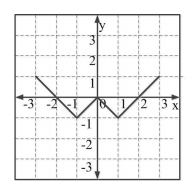
\includegraphics[width=0.4\columnwidth]{GAq9.png}
        \caption*{}
        \label{fig:q9_ga}
    \end{figure}
    \hfill{\brak{\text{GATE XE 2018}}}
    \begin{enumerate}[label=\Alph*)]
        \begin{multicols}{2}
            \item $y = \abs{\abs{x} + 1} - 2$
            \item $y = \abs{\abs{x} - 1} - 1$
            \item $y = \abs{\abs{x} + 1} - 1$
            \item $y = \abs{\abs{x-1} - 1}$
        \end{multicols}
    \end{enumerate}

    \item Consider the following three statements:
    (i) Some roses are red.
    (ii) All red flowers fade quickly.
    (iii) Some roses fade quickly.
    
    Which of the following statements can be logically inferred from the above statements?
    \hfill{\brak{\text{GATE XE 2018}}}
    \begin{enumerate}[label=\Alph*)]
        \item If (i) is true and (ii) is false, then (iii) is false.
        \item If (i) is true and (ii) is false, then (iii) is true.
        \item If (i) and (ii) are true, then (iii) is true.
        \item If (i) and (ii) are false, then (iii) is false.
    \end{enumerate}
\end{enumerate}
\clearpage

\section*{A : ENGINEERING MATHEMATICS (COMPULSORY)}
\begin{enumerate}
    \item The largest interval in which the initial value problem
    \begin{align*}
        e^x \frac{d^2 y}{dx^2} + \frac{1}{\brak{x-5}}\frac{dy}{dx} + \brak{\sqrt{x}}y = \ln\brak{x}, \quad y\brak{1} = 0 \text{ and } \frac{dy}{dx}\brak{1} = 1,
    \end{align*}
    has a unique solution is
    \hfill{\brak{\text{GATE XE 2018}}}
    \begin{enumerate}[label=\Alph*)]
        \begin{multicols}{4}
            \item $\brak{-\infty, \infty}$
            \item $\brak{-5, 5}$
            \item $\brak{0, \infty}$
            \item $\brak{0, 5}$
        \end{multicols}
    \end{enumerate}

    \item The sum of the roots of the indicial equation at $x=0$ of the differential equation
    \begin{align*}
        x^3 \frac{d^2 y}{dx^2} + \brak{x \sin x}\frac{dy}{dx} - \brak{\tan x}y = 0, \quad x > 0,
    \end{align*}
    is
    \hfill{\brak{\text{GATE XE 2018}}}
    \begin{enumerate}[label=\Alph*)]
        \begin{multicols}{4}
            \item 0
            \item 1
            \item 2
            \item -2
        \end{multicols}
    \end{enumerate}

    \item Let $f$ be a three times continuously differentiable real valued function on $\brak{0, 5}$ such that its third derivative $f'''\brak{x} = -\frac{1}{100}$ for all $x \in \brak{0, 5}$. If $P\brak{x}$ is a polynomial of degree $\le 2$ such that $P\brak{1} = f\brak{1}$, $P\brak{2} = f\brak{2}$ and $P\brak{3} = f\brak{3}$ then $\abs{f\brak{4} - P\brak{4}}$ equals \underline{\hspace{2cm}}.
    \hfill{\brak{\text{GATE XE 2018}}}

    \item For real numbers $\alpha_1$ and $\alpha_2$, if the formula $\int_{-1}^{1} f\brak{x} dx = \alpha_1 f\brak{\frac{1}{3}} + \alpha_2 f\brak{-\frac{1}{3}}$ is exact for all polynomials of degree $\le 1$ then $2\alpha_1 + 3\alpha_2$ equals \underline{\hspace{2cm}}.
    \hfill{\brak{\text{GATE XE 2018}}}

    \item Raju has four fair coins and one fair dice. At first Raju tosses a coin. If the coin shows head then he rolls the dice and the number that dice shows is taken as his score. If the coin shows tail then he tosses three more coins and the total number of tails shown (including the first one) is taken as his score. If Raju tells that his score is 2 then the probability that he rolled the dice is (up to two decimal places) \underline{\hspace{2cm}}.
    \hfill{\brak{\text{GATE XE 2018}}}

    \item Let $f$ be a continuously differentiable real valued function defined by
    \begin{align*}
        f\brak{x} = 
        \begin{cases}
            bx+a & \text{if } x < 1, \\
            5x^2 & \text{if } x \ge 1.
        \end{cases}
    \end{align*}
    Then the value of $a^2b$ is \underline{\hspace{2cm}}.
    \hfill{\brak{\text{GATE XE 2018}}}

    \item A rectangular box without top cover having a square base is to be made from a sheet of 108 square meters. Then the largest possible volume of the box in cubic meters is \underline{\hspace{2cm}}.
    \hfill{\brak{\text{GATE XE 2018}}}

    \item Let $A = \myvec{5 & -3 \\ 6 & -4}$. Then the trace of $A^{1000}$ equals
    \hfill{\brak{\text{GATE XE 2018}}}
    \begin{enumerate}[label=\Alph*)]
        \begin{multicols}{4}
            \item $2^{1000} - 1$
            \item $2^{1000} + 1$
            \item 1
            \item $2^{1000}$
        \end{multicols}
    \end{enumerate}

    \item Let $\mathbb{C}$ denote the set of complex numbers and $i^2 = -1$. Let $\gamma$ be the simple positively oriented circle $\abs{z}=1$ and $S = \{z \in \mathbb{C} | 0 < \abs{z} < 2\}$. If $f: S \to \mathbb{C}$ is analytic in $S$ and is given by
    \begin{align*}
        f\brak{z} = \frac{1}{8z^2} - \frac{7}{2z} + \sum_{n=0}^{\infty} a_n z^n, \quad z \in S
    \end{align*}
    then the value of the contour integral $$\frac{1}{\pi i} \oint_\gamma \brak{\frac{e^z}{\cos z} + f\brak{z}} dz$$ is
    \hfill{\brak{\text{GATE XE 2018}}}
    \begin{enumerate}[label=\Alph*)]
        \begin{multicols}{4}
            \item 0
            \item $\frac{1}{8}$
            \item 7
            \item $\frac{7}{2}$
        \end{multicols}
    \end{enumerate}

    \item Let $\mathbb{R}^3$ denote the three dimensional Euclidean space and $\mathbf{F}\brak{x, y, z} = -y\hat{i} + x\hat{j} + z\hat{k}$ for all $\brak{x, y, z} \in \mathbb{R}^3$. If $C$ is the curve described by the parametric equation $\mathbf{r}\brak{t} = \cos t \hat{i} + \sin t \hat{j} + 2t^2\hat{k}, 0 \le t \le 1$, then the value of the line integral $\int_C \mathbf{F} \cdot d\mathbf{r}$ is \underline{\hspace{2cm}}.
    \hfill{\brak{\text{GATE XE 2018}}}

    \item Let $u\brak{x, t}$ satisfy the initial and boundary value problem
    \begin{align*}
        \frac{\partial u}{\partial t} &= 2 \frac{\partial^2 u}{\partial x^2}, \quad 0 < x < \pi, \quad t > 0, \\
        u\brak{0, t} &= 0 = u\brak{\pi, t}, \quad t > 0, \\
        u\brak{x, 0} &= \sin x + 2\sin 4x, \quad 0 < x < \pi.
    \end{align*}
    Then the value of $u\brak{\frac{\pi}{2}, \ln\brak{5}}$ is \underline{\hspace{2cm}}.
    \hfill{\brak{\text{GATE XE 2018}}}
\end{enumerate}
\clearpage

\section*{B : FLUID MECHANICS}
\begin{enumerate}
    \item Rheological diagram of different types of fluids is shown in figure. Column I represents the nature of the fluid and column II represents the curve showing the variation of shear stress against shear strain rate.
    \begin{figure}[H]
        \centering
        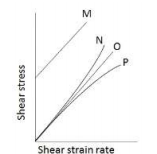
\includegraphics[width=0.5\columnwidth]{q1_fluid_2018.png}
        \caption*{}
        \label{fig:q1_fluid_2018}
    \end{figure}
    \begin{table}[h!] \centering \caption*{} \label{tab:q1_fluid_2018}
        \begin{tabular}{ll}
            \textbf{Column I} & \textbf{Column II} \\
            (i) Newtonian & M \\
            (ii) Shear thinning & N \\
            (iii) Shear thickening & O \\
            (iv) Bingham plastic & P \\
        \end{tabular}
    \end{table}
    The most appropriate match between columns I and II is,
    \hfill{\brak{\text{GATE XE 2018}}}
    \begin{enumerate}[label=\Alph*)]
        \item (i) - O; (ii) - N ; (iii) - P; (iv) - M
        \item (i) - O; (ii) - P ; (iii) - N; (iv) - M
        \item (i) - P; (ii) - O ; (iii) - M; (iv) - N
        \item (i) - P; (ii) - O ; (iii) - N; (iv) - M
    \end{enumerate}

    \item In a two-dimensional, incompressible and irrotational flow, stream function ($\psi = \psi(x, y)$) and velocity potential ($\phi = \phi(x, y)$) exist. The velocities in x and y directions are non-zero. The product of $\left.\frac{dy}{dx}\right|_{\phi=\text{constant}}$ and $\left.\frac{dy}{dx}\right|_{\psi=\text{constant}}$, is
    \hfill{\brak{\text{GATE XE 2018}}}
    \begin{enumerate}[label=\Alph*)]
        \begin{multicols}{4}
            \item -1
            \item 0
            \item 1
            \item $\infty$
        \end{multicols}
    \end{enumerate}

    \item The inviscid flow past a rotating circular cylinder can be generated by the superposition of
    \hfill{\brak{\text{GATE XE 2018}}}
    \begin{enumerate}[label=\Alph*)]
        \item uniform flow, source and vortex
        \item uniform flow, doublet
        \item uniform flow, sink and vortex
        \item uniform flow, doublet and vortex
    \end{enumerate}

    \item The velocity field and the surface normal vector are given by, $\vec{V} = u\hat{i} + v\hat{j} + w\hat{k}$ and $\vec{n} = n_1\hat{i} + n_2\hat{j} + n_3\hat{k}$, respectively. If Euler equations are to be solved, the boundary condition that must be satisfied at the wall is,
    \hfill{\brak{\text{GATE XE 2018}}}
    \begin{enumerate}[label=\Alph*)]
        \begin{multicols}{4}
            \item $\vec{V} \cdot \vec{n} = 0$
            \item $\vec{V} = 0$
            \item $\nabla \cdot \vec{V} = 0$
            \item $\vec{V} \times \vec{n} = 0$
        \end{multicols}
    \end{enumerate}

    \item The influence of Froude number is most significant in
    \hfill{\brak{\text{GATE XE 2018}}}
    \begin{enumerate}[label=\Alph*)]
        \begin{multicols}{2}
            \item capillary flows
            \item creeping flows
            \item free surface flows
            \item compressible flows
        \end{multicols}
    \end{enumerate}

    \item If the stream function ($\psi(x,y)$) for a two-dimensional incompressible flow field is given as $2y(x^2 - y^2)$, the corresponding velocity field is
    \hfill{\brak{\text{GATE XE 2018}}}
    \begin{enumerate}[label=\Alph*)]
        \item $\vec{V} = 2(x^2 - 3y^2)\hat{i} + 4xy\hat{j}$
        \item $\vec{V} = 2(x^2 - 3y^2)\hat{i} - 4xy\hat{j}$
        \item $\vec{V} = 2(x^2y)\hat{i} - 4xy\hat{j}$
        \item $\vec{V} = 2(x^2y)\hat{i} + 4xy\hat{j}$
    \end{enumerate}

    \item Water is flowing in two different tubes of diameters D and 2D, with the same velocity. The ratio of laminar friction factors for the larger diameter tube to the smaller diameter tube is
    \hfill{\brak{\text{GATE XE 2018}}}
    \begin{enumerate}[label=\Alph*)]
        \begin{multicols}{4}
            \item 0.5
            \item 1.0
            \item 2.0
            \item 4.0
        \end{multicols}
    \end{enumerate}

    \item If the velocity field is $\vec{V} = xy^2\hat{i} + 4xy\hat{j}$ m/s, vorticity of the fluid element in the field at (x=1, y=2) in s$^{-1}$ is \underline{\hspace{2cm}}.
    \hfill{\brak{\text{GATE XE 2018}}}

    \item A pitot-static tube is used to measure air velocity in a duct by neglecting losses. The density of air is 1.2 kg/m$^3$. If the difference between the total and static pressures is 1 kPa, the velocity of air at the measuring location, in m/s, is \underline{\hspace{2cm}}.
    \hfill{\brak{\text{GATE XE 2018}}}

    \item A parallelepiped of (2 m $\times$ 2 m) square cross-section and 10 m in length, is partially floating in water upto a depth of 1.2 m, with its longest side being horizontal. The specific gravity of the block is
    \hfill{\brak{\text{GATE XE 2018}}}
    \begin{enumerate}[label=\Alph*)]
        \begin{multicols}{4}
            \item 0.8
            \item 0.6
            \item 0.5
            \item 0.4
        \end{multicols}
    \end{enumerate}

    \item The velocity field in a two-dimensional, unsteady flow is given by $\vec{V}(x,y,t) = 2xy^2\hat{i} + 3xyt\hat{j}$ m/s. The magnitude of acceleration of a fluid particle located at x=1 m, y=1 m at the time t=1 s, in m/s$^2$, is
    \hfill{\brak{\text{GATE XE 2018}}}
    \begin{enumerate}[label=\Alph*)]
        \begin{multicols}{4}
            \item 16.0
            \item 18.1
            \item 24.1
            \item 34.1
        \end{multicols}
    \end{enumerate}

    \item In a two-dimensional, incompressible and irrotational flow, fluid velocity (v) in the y-direction is given by $v = 2x - 5y$. The velocity (u) in the x-direction is
    \hfill{\brak{\text{GATE XE 2018}}}
    \begin{enumerate}[label=\Alph*)]
        \begin{multicols}{4}
            \item $u = 2x - 5y$
            \item $u = 2x + 5y$
            \item $u = 5x + 2y$
            \item $u = 5x - 2y$
        \end{multicols}
    \end{enumerate}

    \item A two-dimensional laminar viscous liquid film of constant thickness (h) steadily flows down an incline as shown in figure. Acceleration due to gravity is g. If the velocity profile in the liquid film is given as, $u = ky(2h-y); v=0$, the value of constant $k$ is
    \begin{figure}[H] \centering 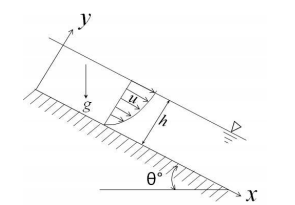
\includegraphics[width=0.6\columnwidth]{q13_fluid_2018.png} \caption*{} \label{fig:q13_fluid_2018} \end{figure}
    \hfill{\brak{\text{GATE XE 2018}}}
    \begin{enumerate}[label=\Alph*)]
        \begin{multicols}{2}
            \item $\frac{\rho g \sin\theta}{2\mu}$
            \item $\frac{\rho g \cos\theta}{2\mu}$
            \item $\rho g \sin\theta$
            \item $\rho g \cos\theta$
        \end{multicols}
    \end{enumerate}

    \item A water jet of 100 mm diameter issuing out of a nozzle at a speed of 50 m/s strikes a vane and flows along it as shown in figure. The vane is attached to a cart which is moving at a constant speed of 20 m/s on a frictionless track. The jet is deflected at an angle of 30$\degree$. Take the density of water as 1000 kg/m$^3$. Neglecting the friction between the vane and the fluid, the magnitude of the force exerted by water on the cart in the x-direction, in N, is \underline{\hspace{2cm}}.
    \begin{figure}[H] \centering 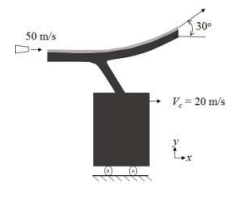
\includegraphics[width=0.5\columnwidth]{q14_fluid_2018.png} \caption*{} \label{fig:q14_fluid_2018} \end{figure}
    \hfill{\brak{\text{GATE XE 2018}}}

    \item Capillary waves are generated in the sea. The speed of propagation (C) of these waves is known to be a function of density ($\rho$), wave length ($\lambda$), and surface tension ($\sigma$). Assume, $\rho$ and $\lambda$ to be constant. If the surface tension is doubled, in the functional form of the relevant non-dimensional group, the percentage increase in propagation speed (C) is \underline{\hspace{2cm}}.
    \hfill{\brak{\text{GATE XE 2018}}}

    \item Consider a fully developed, two-dimensional and steady flow of a viscous fluid between two fixed parallel plates separated by a distance of 30 mm. The dynamic viscosity of the fluid is 0.01 kg/m-s and the pressure drop per unit length is 300 Pa/m. The fluid velocity at a distance of 10 mm from the bottom plate, in m/s, is \underline{\hspace{2cm}}.
    \hfill{\brak{\text{GATE XE 2018}}}

    \item A 2.6 gram smooth table-tennis (ping-pong) ball has a diameter of 38 mm. Density ($\rho$) of air is 1.2 kg/m$^3$. Neglect the effect of gravity. Take coefficient of drag as 0.5. If the ball is struck with an initial velocity of 30 m/s, the initial deceleration, in m/s$^2$, is \underline{\hspace{2cm}}.
    \hfill{\brak{\text{GATE XE 2018}}}

    \item On a flat plate, transition from laminar to turbulent boundary layer occurred at a critical Reynolds number ($Re_{cr}$). The empirical relations for the laminar and turbulent boundary layer thickness are given by $\frac{\delta_{lam}}{x} = 5.48 Re_x^{-0.5}$ and $\frac{\delta_{turb}}{x} = 0.37 Re_x^{-0.2}$, respectively. The ratio of laminar to turbulent boundary layer thickness, at the location of transition, is 0.3. The value of $Re_{cr}$ is \underline{\hspace{2cm}}.
    \hfill{\brak{\text{GATE XE 2018}}}

    \item In a capillary tube of radius $R = 0.25$ mm, a fully developed laminar velocity profile is defined as, $u = -\frac{R^2}{4\mu}\brak{\frac{dp}{dx}}\brak{1-\frac{r^2}{R^2}}$. In this expression, $-\frac{dp}{dx} = 1$ MPa/m, $\mu$ is the dynamic viscosity of the fluid, and $r$ is the radial position from the centerline of the tube. If the flow rate through the tube is 1000 mm$^3$/s, the viscosity of the fluid, in Pa-s, is \underline{\hspace{2cm}}.
    \hfill{\brak{\text{GATE XE 2018}}}

    \item The skin friction coefficient for a turbulent pipe flow is defined as, $C_f = \frac{\tau_w}{1/2 \rho V^2}$, where $\tau_w$ is the wall shear stress and $V$ is the average flow velocity. The value of $C_f$ is empirically given by the relation: $C_f = 0.065(2/Re)^{0.25}$, where $Re$ is the Reynolds number. If the average flow velocity is 10 m/s, diameter of the pipe is 250 mm, kinematic viscosity of the fluid is $0.25 \times 10^{-6}$ m$^2$/s, and density of the fluid is 700 kg/m$^3$, the skin friction drag induced by the flow over 1 m length of the pipe, in N, is \underline{\hspace{2cm}}.
    \hfill{\brak{\text{GATE XE 2018}}}

    \item A (150 mm $\times$ 150 mm) square pillar is located in a river with water flowing at a velocity of 2 m/s, as shown in figure. The height of the pillar in water is 8 m. Take density of water as 1000 kg/m$^3$ and kinematic viscosity as $1 \times 10^{-6}$ m$^2$/s$^2$. The coefficient of drag of the pillar is 2.0. The drag force exerted by water on the pillar in N is \underline{\hspace{2cm}}.
    \begin{figure}[H] \centering 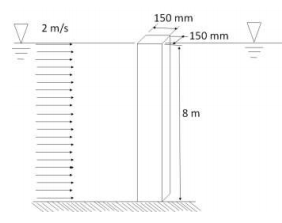
\includegraphics[width=0.5\columnwidth]{q21_fluid_2018.png} \caption*{} \label{fig:q21_fluid_2018} \end{figure}
    \hfill{\brak{\text{GATE XE 2018}}}

    \item An orifice plate is used to measure flow rate of air (density = 1.23 kg/m$^3$) in a duct of 250 mm diameter as shown in figure. The volume flow rate is 1 m$^3$/s. Flow at sections 1 and 3 is uniform and section 2 is located at vena contracta. The diameter ratio, $D_t/D_1$, is 0.66. The flow area at vena contracta, $A_2 = 0.65 A_t$, where $A_t$ is area of the orifice. The pressure difference between locations 2 and 3 in N/m$^2$ is \underline{\hspace{2cm}}.
    \begin{figure}[H] \centering 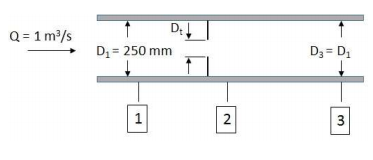
\includegraphics[width=0.7\columnwidth]{q22_fluid_2018.png} \caption*{} \label{fig:q22_fluid_2018} \end{figure}
    \hfill{\brak{\text{GATE XE 2018}}}
\end{enumerate}
\clearpage

\section*{C: MATERIALS SCIENCES}
\begin{enumerate}
    \item The stress ratio for a completely reversed cyclic loading during a fatigue test is
    \hfill{\brak{\text{GATE XE 2018}}}
    \begin{enumerate}[label=\Alph*)]
        \begin{multicols}{4}
            \item 0
            \item 1
            \item -1
            \item -1/2
        \end{multicols}
    \end{enumerate}

    \item Minimum symmetry that a cubic crystal must possess is
    \hfill{\brak{\text{GATE XE 2018}}}
    \begin{enumerate}[label=\Alph*)]
        \item four 3-fold rotation axes.
        \item three 4-fold rotation axes.
        \item three orthogonal mirror planes.
        \item centre of symmetry.
    \end{enumerate}

    \item If a material is repelled in an external magnetic field then it is
    \hfill{\brak{\text{GATE XE 2018}}}
    \begin{enumerate}[label=\Alph*)]
        \begin{multicols}{2}
            \item Ferromagnetic
            \item Diamagnetic
            \item Paramagnetic
            \item Antiferromagnetic
        \end{multicols}
    \end{enumerate}

    \item An electron makes a transition from the valence band to the conduction band in an indirect band gap semiconductor. Which one of the following is true?
    \hfill{\brak{\text{GATE XE 2018}}}
    \begin{enumerate}[label=\Alph*)]
        \item Energy of the electron decreases.
        \item A photon is emitted in the process.
        \item A phonon is annihilated in the process.
        \item A photon is created in the process.
    \end{enumerate}

    \item Which one of the following is the characteristic of a screw dislocation?
    \hfill{\brak{\text{GATE XE 2018}}}
    \begin{enumerate}[label=\Alph*)]
        \item Dislocation line and Burgers vector are parallel.
        \item Direction of motion of dislocation is parallel to the Burgers vector.
        \item Atomic displacement due to the movement of the dislocation is in the direction of the motion of the dislocation line.
        \item It has a unique slip plane.
    \end{enumerate}

    \item The number of vibrational degrees of freedom for a non-linear triatomic molecule are
    \hfill{\brak{\text{GATE XE 2018}}}
    \begin{enumerate}[label=\Alph*)]
        \begin{multicols}{4}
            \item 9
            \item 6
            \item 4
            \item 3
        \end{multicols}
    \end{enumerate}

    \item An atom is restricted to move in one dimension by making unit jumps either to the left or right, as shown in the figure. Assuming that a jump to the left or right is equally probable, the probability of the atom returning back to the starting point after four jumps is
    \begin{figure}[H] \centering 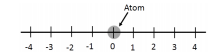
\includegraphics[width=0.6\columnwidth]{q7_material_2018.png} \caption*{} \label{fig:q7_material_2018} \end{figure}
    \hfill{\brak{\text{GATE XE 2018}}}
    \begin{enumerate}[label=\Alph*)]
        \begin{multicols}{4}
            \item 0.250
            \item 0.333
            \item 0.375
            \item 0.500
        \end{multicols}
    \end{enumerate}

    \item For a two-dimensional solid, the variation of lattice specific heat as a function of temperature $T$ (in K, at low temperatures) is given as: $C_p = bT^n$, where $b$ is a constant. The value of $n$ is \underline{\hspace{2cm}}.
    \hfill{\brak{\text{GATE XE 2018}}}

    \item If the cation (C) to anion (A) radius ratio, $r_C/r_A$ is 0.6, then the coordination number (i.e., number of A ions surrounding a C ion) is likely to be \underline{\hspace{2cm}}.
    \hfill{\brak{\text{GATE XE 2018}}}

    \item Match the invariant reactions in Column I with the names in Column II (L is liquid phase, and $\alpha, \beta, \gamma$ are solid phases). All reactions proceed to the right on cooling.
    \begin{table}[h!] \centering \caption*{} \label{tab:q10_material_2018}
        \begin{tabular}{ll}
            \textbf{Column I} & \textbf{Column II} \\
            (P) $L \rightleftharpoons \alpha + \beta$ & (1) Monotectic \\
            (Q) $L + \alpha \rightleftharpoons \beta$ & (2) Peritectoid \\
            (R) $\gamma \rightleftharpoons \alpha + \beta$ & (3) Peritectic \\
            (S) $\alpha + \beta \rightleftharpoons \gamma$ & (4) Eutectoid \\
            & (5) Eutectic \\
        \end{tabular}
    \end{table}
    \hfill{\brak{\text{GATE XE 2018}}}
    \begin{enumerate}[label=\Alph*)]
        \begin{multicols}{2}
            \item P-5, Q-1, R-4, S-3
            \item P-5, Q-3, R-4, S-2
            \item P-5, Q-1, R-2, S-4
            \item P-2, Q-1, R-4, S-5
        \end{multicols}
    \end{enumerate}

    \item Consider the following anodic (oxidation) reaction in an acidic solution:
    \begin{align*}
        Mg \rightarrow Mg^{+2} + 2e^-
    \end{align*}
    If 48250 Coulomb charge is produced during this anodic reaction then the amount of Mg (in g) dissolved into the solution is \underline{\hspace{2cm}}.
    (Given: Faraday Constant = 96500 C/mole of electrons, Atomic weight of Mg = 24)
    \hfill{\brak{\text{GATE XE 2018}}}
    \begin{enumerate}[label=\Alph*)]
        \begin{multicols}{4}
            \item 6
            \item 12
            \item 24
            \item 48
        \end{multicols}
    \end{enumerate}

    \item An intrinsic semiconductor has conduction electron concentration, $n = 10^{12}$ cm$^{-3}$. The mobility of both electrons and holes are identical $= 4 \times 10^4$ cm$^2$ V$^{-1}$ s$^{-1}$. If a voltage of 100 V is applied on two parallel end faces of the cube (edge length 1 cm) through Ohmic contacts, the current through the cube would be (in mA) \underline{\hspace{2cm}}.
    (Given: charge of electron = $1.6 \times 10^{-19}$ C)
    \hfill{\brak{\text{GATE XE 2018}}}
    \begin{enumerate}[label=\Alph*)]
        \begin{multicols}{4}
            \item 640
            \item 1280
            \item 6400
            \item 12800
        \end{multicols}
    \end{enumerate}

    \item An infinite plate with a through-thickness crack of length 2 mm is subjected to a tensile stress (as shown in the figure). Assuming the plate to be linear elastic, the fracture stress is \underline{\hspace{2cm}} MPa (round off to the nearest whole number).
    (Given: Fracture toughness, $K_{IC} = 25$ MPa $\sqrt{m}$)
    \begin{figure}[H] \centering 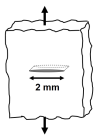
\includegraphics[width=0.3\columnwidth]{q13_material_2018.png} \caption*{} \label{fig:q13_material_2018} \end{figure}
    \hfill{\brak{\text{GATE XE 2018}}}

    \item A unidirectionally aligned carbon fibre reinforced epoxy composite is loaded as shown in the figure. The volume fraction of the fibre is 0.6. The Young's modulus of the composite is \underline{\hspace{2cm}} GPa.
    (Given: Young's Modulus of the fibre and the matrix are 200 GPa and 10 GPa, respectively)
    \begin{figure}[H] \centering 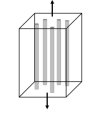
\includegraphics[width=0.3\columnwidth]{q14_material_2018.png} \caption*{} \label{fig:q14_material_2018} \end{figure}
    \hfill{\brak{\text{GATE XE 2018}}}

    \item A sintered sample was weighed in air and water using an analytical balance. The mass of the sample in air is 2.67 g and its apparent mass in water is 1.67 g. The density of the sample is \underline{\hspace{2cm}} g cm$^{-3}$ (give answer up to 2 decimal places).
    (Given: Density of water = 1.00 g cm$^{-3}$)
    \hfill{\brak{\text{GATE XE 2018}}}

    \item The atoms in a gas laser have two energy levels such that a transition from the higher to the lower level releases a photon of wavelength 500 nm. If $7 \times 10^{20}$ atoms are pumped into the upper level with $4 \times 10^{20}$ atoms in the lower level, the amount of energy released in a single pulse is \underline{\hspace{2cm}} Joules (give answer up to 2 decimal places).
    (Given: Planck's constant, $h = 6.6 \times 10^{-34}$ J s; speed of light, $c = 3 \times 10^8$ m s$^{-1}$)
    \hfill{\brak{\text{GATE XE 2018}}}

    \item The speed of an electron is measured to be 300 m s$^{-1}$ with an uncertainty of 0.01\%. The fundamental accuracy with which the position of the electron can be determined simultaneously with the speed in the same experiment is \underline{\hspace{2cm}} mm (give answer up to 2 decimal places).
    (Given: Planck's constant, $h = 6.6 \times 10^{-34}$ J s; mass of electron = $9.1 \times 10^{-31}$ kg)
    \hfill{\brak{\text{GATE XE 2018}}}

    \item When 3 identical non-interacting spin ½ particles are put in an infinite potential well, the ground state energy of the system is 18 meV. If instead, seven particles are put inside the potential well, the new ground state energy is \underline{\hspace{2cm}} meV.
    \hfill{\brak{\text{GATE XE 2018}}}

    \item If the value of the integral (I) is 4, the value of the constant b is \underline{\hspace{2cm}} (give answer up to 2 decimal places).
    \begin{align*}
        I = \int_{-\infty}^{\infty} e^{-\frac{x^2}{b}} dx
    \end{align*}
    \hfill{\brak{\text{GATE XE 2018}}}

    \item X-ray diffraction pattern is obtained from FCC polycrystalline aluminium (lattice parameter = 0.405 nm) using Cr-K$\alpha$ radiation of wavelength 0.229 nm. The maximum number of peaks that can be observed in the pattern is \underline{\hspace{2cm}}.
    \hfill{\brak{\text{GATE XE 2018}}}

    \item The planar atomic density in the (110) plane of a BCC iron crystal is \underline{\hspace{2cm}} nm$^{-2}$ (give answer up to 2 decimal places).
    (Given: lattice parameter of iron is 0.287 nm)
    \hfill{\brak{\text{GATE XE 2018}}}

    \item Mild steel is carburized at 1300 K for 1 hour to obtain a certain case depth. Keeping the time as 1 hour, the case depth can be doubled by increasing the temperature to \underline{\hspace{2cm}} K (round off to the nearest whole number).
    (Given: Activation energy Q = 148 kJ mol$^{-1}$, Gas constant, R = 8.314 J mol$^{-1}$ K$^{-1}$)
    \hfill{\brak{\text{GATE XE 2018}}}
\end{enumerate}
\clearpage

\section*{D: SOLID MECHANICS}
\begin{enumerate}
    \item A thin cylinder (thickness, t and diameter, d) with closed ends is subjected to an internal pressure, p. The ratio of hoop stress to longitudinal stress developed in the wall of the cylinder is
    \hfill{\brak{\text{GATE XE 2018}}}
    \begin{enumerate}[label=\Alph*)]
        \begin{multicols}{4}
            \item 1:4
            \item 1:2
            \item 1:1
            \item 2:1
        \end{multicols}
    \end{enumerate}

    \item A steel rod is fixed at one end and free at the other end. The coefficient of thermal expansion of the steel is $\alpha$, and modulus of elasticity is $E$. If the temperature of the rod is increased by $\Delta T$ then the stress and strain developed in the rod are respectively
    \hfill{\brak{\text{GATE XE 2018}}}
    \begin{enumerate}[label=\Alph*)]
        \item zero, $\alpha\Delta T$
        \item $E\alpha\Delta T$, $\alpha\Delta T$
        \item $E\alpha\Delta T$, zero
        \item zero, zero
    \end{enumerate}

    \item The effective lengths of the columns with ideal boundary conditions shown in Case-I, Case-II, and Case-III are respectively
    \begin{figure}[H] \centering 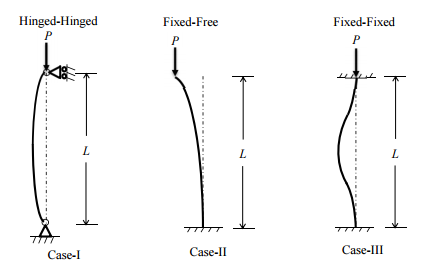
\includegraphics[width=\columnwidth]{q3_solid.png} \caption*{} \label{fig:q3_solid} \end{figure}
    \hfill{\brak{\text{GATE XE 2018}}}
    \begin{enumerate}[label=\Alph*)]
        \item L, 4L, 2L
        \item L, 2L, L/4
        \item L, L, L
        \item L, 2L, L/2
    \end{enumerate}

    \item At a point in a stressed body, sum of the normal stresses acting on perpendicular faces of an arbitrarily oriented plane stress element is always
    \hfill{\brak{\text{GATE XE 2018}}}
    \begin{enumerate}[label=\Alph*)]
        \item dependent on the angle of orientation of the element
        \item constant and independent of angle of orientation of the element
        \item one half of the sum of the principal stresses
        \item zero
    \end{enumerate}

    \item The principal stresses on a plane stress element are shown in the figure. The maximum shear stress (in MPa) is
    \begin{figure}[H] \centering 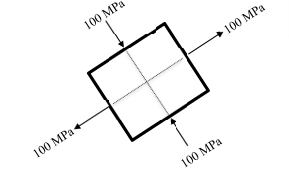
\includegraphics[width=0.4\columnwidth]{q5_solid.png} \caption*{} \label{fig:q5_solid} \end{figure}
    \hfill{\brak{\text{GATE XE 2018}}}
    \begin{enumerate}[label=\Alph*)]
        \begin{multicols}{4}
            \item 200
            \item 100
            \item 50
            \item 0
        \end{multicols}
    \end{enumerate}

    \item A rigid and thin L-shaped bracket is fixed to the wall at point B, and a force F is applied at point A as shown. For a given force F, the point B experiences the maximum clockwise moment when the inclination $\theta$ (in degrees) with the x-axis is \underline{\hspace{2cm}} [up to two decimal places].
    \begin{figure}[H] \centering 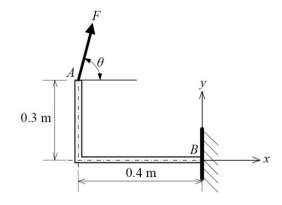
\includegraphics[width=0.5\columnwidth]{q6_solid.png} \caption*{} \label{fig:q6_solid} \end{figure}
    \hfill{\brak{\text{GATE XE 2018}}}

    \item A cantilever beam with length, L = 1 m, modulus of elasticity, E = 210 GPa, and area moment of inertia, $I = 1.2 \times 10^{-7}$ m$^4$ carries a concentrated mass m = 100 kg at its free-end. By idealizing it as a single degree-of-freedom system and neglecting the mass of the cantilever beam, the natural frequency (in rad/s) of small transverse oscillations of the mass m is \underline{\hspace{2cm}} [up to two decimal places].
    \hfill{\brak{\text{GATE XE 2018}}}

    \item For a typical grade of steel, the value of modulus of elasticity (E) and Poisson's ratio ($\nu$) are 208 GPa and 0.3 respectively. The value of shear modulus (G) of the steel (in GPa) is \underline{\hspace{2cm}}.
    \hfill{\brak{\text{GATE XE 2018}}}

    \item A tensile test is performed on a metallic specimen of diameter 8 mm and gauge length 50 mm. When the tensile load P reaches a value of 20 kN, the distance between the gauge marks increases by 0.09 mm. If the sample remains within the elastic limit, the modulus of elasticity (in GPa) of the test metal is \underline{\hspace{2cm}} [up to two decimal places].
    \begin{figure}[H] \centering 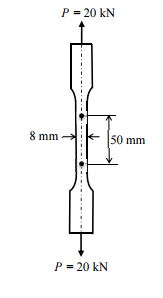
\includegraphics[width=0.3\columnwidth]{q9_solid.png} \caption*{} \label{fig:q9_solid} \end{figure}
    \hfill{\brak{\text{GATE XE 2018}}}

    \item A beam ABC is subjected to load P at its free end C as shown in the figure. The flexural rigidity of the beam is EI. The vertical support reaction at point B is
    \begin{figure}[H] \centering 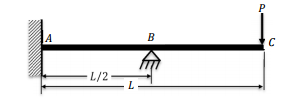
\includegraphics[width=0.6\columnwidth]{q10_solid.png} \caption*{} \label{fig:q10_solid} \end{figure}
    \hfill{\brak{\text{GATE XE 2018}}}
    \begin{enumerate}[label=\Alph*)]
        \begin{multicols}{4}
            \item $\frac{5P}{4}$
            \item $\frac{5P}{2}$
            \item $\frac{4P}{5}$
            \item $\frac{2P}{5}$
        \end{multicols}
    \end{enumerate}

    \item A horizontal effort P is applied to raise a block of weight W on a rough surface inclined at an angle $\theta$ with the horizontal. If $\mu_s$ is the coefficient of static friction between the block and the surface, the minimum effort P required to impend the upward motion of the block along the surface is
    \begin{figure}[H] \centering 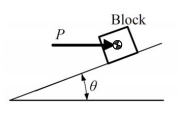
\includegraphics[width=0.4\columnwidth]{q11_solid.png} \caption*{} \label{fig:q11_solid} \end{figure}
    \hfill{\brak{\text{GATE XE 2018}}}
    \begin{enumerate}[label=\Alph*)]
        \begin{multicols}{4}
            \item $W \brak{\frac{\mu_s - \tan\theta}{1+\mu_s\tan\theta}}$
            \item $W \brak{\frac{\mu_s + \tan\theta}{1-\mu_s\tan\theta}}$
            \item $W \brak{\frac{\mu_s - \tan\theta}{1-\mu_s\tan\theta}}$
            \item $W \brak{\frac{\mu_s + \tan\theta}{1+\mu_s\tan\theta}}$
        \end{multicols}
    \end{enumerate}

    \item Three round bars of same material, equal lengths, and different cross-sectional dimensions are shown in the figures as Case-I, Case-II and Case-III. All the bars are clamped at the upper end, and a concentrated load P is applied at the lower end of each bar. If the elastic strain energy stored in the bar shown in Case-I is $U_1$ then the elastic strain energy stored in Case-II and Case-III respectively is
    \begin{figure}[H] \centering 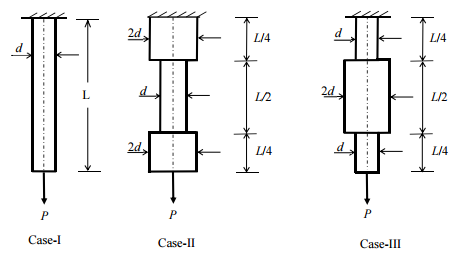
\includegraphics[width=\columnwidth]{q12_solid.png} \caption*{} \label{fig:q12_solid} \end{figure}
    \hfill{\brak{\text{GATE XE 2018}}}
    \begin{enumerate}[label=\Alph*)]
        \begin{multicols}{2}
            \item $\brak{8/5}U_1, \brak{5/8}U_1$
            \item $\brak{5/16}U_1, \brak{5/16}U_1$
            \item $\brak{5/8}U_1, \brak{8/5}U_1$
            \item $\brak{5/8}U_1, \brak{5/8}U_1$
        \end{multicols}
    \end{enumerate}

    \item A rigid uniform rod with mass m, length L and center of gravity G is freely suspended from a hinge as shown in the figure. The rod is given a small angular displacement $\theta$ in the counter-clockwise direction from the position in which it hangs vertically ($\theta = 0$). If g is the acceleration due to gravity, the natural frequency of oscillations (in rad/s) is
    \begin{figure}[H] \centering 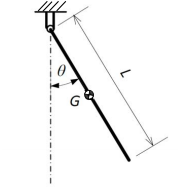
\includegraphics[width=0.4\columnwidth]{q13_solid.png} \caption*{} \label{fig:q13_solid} \end{figure}
    \hfill{\brak{\text{GATE XE 2018}}}
    \begin{enumerate}[label=\Alph*)]
        \begin{multicols}{4}
            \item $\sqrt{\frac{6g}{L}}$
            \item $\sqrt{\frac{2g}{L}}$
            \item $\sqrt{\frac{3g}{2L}}$
            \item $\sqrt{\frac{g}{L}}$
        \end{multicols}
    \end{enumerate}

    \item A cylindrical member, made up of ductile material, is subjected to pure torsion as shown in the figure. The failure plane (from Option-I to Option-IV) for ductile material as per maximum shear stress theory is represented by
    \begin{figure}[H] \centering 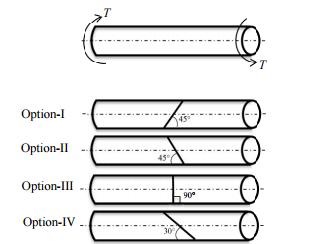
\includegraphics[width=0.6\columnwidth]{q14_solid.png} \caption*{} \label{fig:q14_solid} \end{figure}
    \hfill{\brak{\text{GATE XE 2018}}}
    \begin{enumerate}[label=\Alph*)]
        \item Option I
        \item Option II
        \item Option III
        \item Option IV
    \end{enumerate}

    \item A simply supported beam of span L is subjected to a couple $M_o$ at a distance a from support A. Among the four options (Option-I to Option-IV) shown, the correct shear force diagram of the beam is
    \begin{figure}[H] \centering 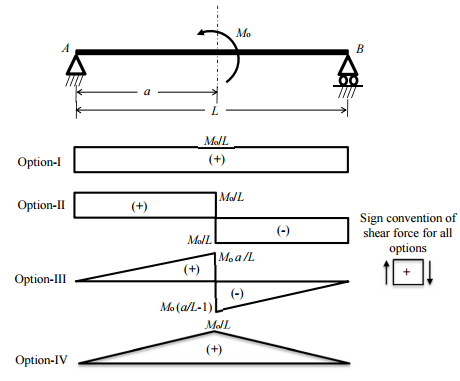
\includegraphics[width=0.8\columnwidth]{q15_solid.png} \caption*{} \label{fig:q15_solid} \end{figure}
    \hfill{\brak{\text{GATE XE 2018}}}
    \begin{enumerate}[label=\Alph*)]
        \begin{multicols}{4}
            \item Option-I
            \item Option-II
            \item Option-III
            \item Option-IV
        \end{multicols}
    \end{enumerate}

    \item A circular shaft ABC of diameter, d and length, L is fixed at end A. It is subjected to the torsional moments at point B and point C as shown in the figure. The ratio of angle of twists at point B to point C is
    \begin{figure}[H] \centering 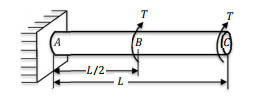
\includegraphics[width=0.6\columnwidth]{q16_solid.png} \caption*{} \label{fig:q16_solid} \end{figure}
    \hfill{\brak{\text{GATE XE 2018}}}
    \begin{enumerate}[label=\Alph*)]
        \begin{multicols}{4}
            \item 1.5 : 1
            \item 1 : 3
            \item 1 : 2
            \item 1 : 1.5
        \end{multicols}
    \end{enumerate}

    \item A circular steel bar of diameter 10 mm is bent into the shape as shown in figure, and lies in x-z plane. A horizontal force P is applied along the positive z-direction as shown. The yield strength of the steel is 200 MPa. Neglecting the effect of transverse shear, the load P (in Newton) required to initiate yielding as per maximum shear stress theory of failure is \underline{\hspace{2cm}} [up to two decimal places].
    \begin{figure}[H] \centering 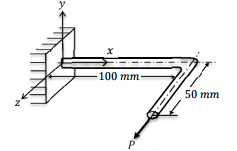
\includegraphics[width=0.5\columnwidth]{q17_solid.png} \caption*{} \label{fig:q17_solid} \end{figure}
    \hfill{\brak{\text{GATE XE 2018}}}

    \item Two sliders A and B, connected by a rigid link of length L, slide in two mutually perpendicular and frictionless guide-ways. At a particular instance, the slider A is moving in the downward direction with a speed of 0.05 m/s. At this instance, the magnitude of the velocity of slider B (in m/s) is \underline{\hspace{2cm}} [up to two decimal places].
    \begin{figure}[H] \centering 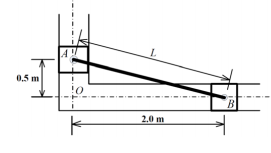
\includegraphics[width=0.6\columnwidth]{q18_solid.png} \caption*{} \label{fig:q18_solid} \end{figure}
    \hfill{\brak{\text{GATE XE 2018}}}

    \item A simply supported beam ABC is subjected to load as shown in the figure. The 20 kN load is applied at point B with the help of a welded bracket as shown. The beam has a rectangular cross-section of 15 mm width and 100 mm depth as shown. The maximum transverse shear stress developed in the beam (in MPa) is \underline{\hspace{2cm}} [up to one decimal place].
    \begin{figure}[H] \centering 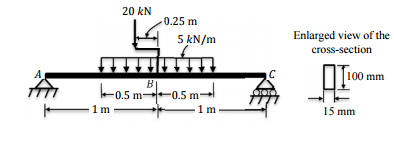
\includegraphics[width=0.8\columnwidth]{q19_solid.png} \caption*{} \label{fig:q19_solid} \end{figure}
    \hfill{\brak{\text{GATE XE 2018}}}

    \item A rigid rod ABC, in the form of a quarter-circular arc of radius R, is hinged at C and supported by a roller at B. A vertical force P is applied at the end A of the bar. For the reactions at B and C to be equal in magnitude, the value of the angle $\theta$ (in degrees) is \underline{\hspace{2cm}} [up to two decimal places].
    \begin{figure}[H] \centering 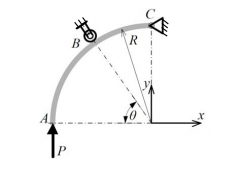
\includegraphics[width=0.4\columnwidth]{q20_solid.png} \caption*{} \label{fig:q20_solid} \end{figure}
    \hfill{\brak{\text{GATE XE 2018}}}

    \item A marble of mass m slides along a frictionless linear slide AB kept in a vertical plane. The marble is released from point A with zero initial velocity, and it reaches point B under the action of gravity. Assuming the acceleration due to gravity to be 9.81 m/s$^2$, the speed (in m/s) of the marble when it just reaches point B is \underline{\hspace{2cm}} [up to two decimal places].
    \begin{figure}[H] \centering 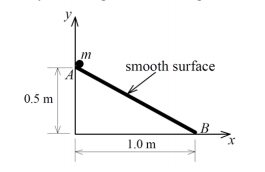
\includegraphics[width=0.4\columnwidth]{q21_solid.png} \caption*{} \label{fig:q21_solid} \end{figure}
    \hfill{\brak{\text{GATE XE 2018}}}

    \item A horizontal force 10 N is applied at support B on the frame as shown in figure. Considering only bending deformation, the vertical reaction (in N) at support B is \underline{\hspace{2cm}} [up to one decimal place].
    \begin{figure}[H] \centering 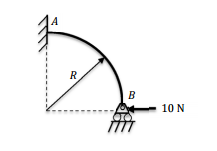
\includegraphics[width=0.3\columnwidth]{q22_solid.png} \caption*{} \label{fig:q22_solid} \end{figure}
    \hfill{\brak{\text{GATE XE 2018}}}
\end{enumerate}
\clearpage

\section*{E : THERMODYNAMICS}
\begin{enumerate}
    \item When a fixed mass of air-water vapour mixture is heated at constant pressure,
    \hfill{\brak{\text{GATE XE 2018}}}
    \begin{enumerate}[label=\Alph*)]
        \item both relative and specific humidity decrease.
        \item relative humidity decreases, but specific humidity remains unchanged.
        \item specific humidity decreases, but relative humidity remains unchanged.
        \item both relative and specific humidity increase.
    \end{enumerate}

    \item For a reversible isothermal expansion of one mole of an ideal gas from state 1 to state 2, the magnitude of work done is
    \hfill{\brak{\text{GATE XE 2018}}}
    \begin{enumerate}[label=\Alph*)]
        \begin{multicols}{2}
            \item $RT \ln \brak{\frac{P_1}{P_2}}$
            \item $P_1V_2 - P_2V_1$
            \item $R \ln \brak{\frac{V_1}{V_2}}$
            \item 0
        \end{multicols}
    \end{enumerate}

    \item The statement which is NOT a consequence of the first law of thermodynamics is
    \hfill{\brak{\text{GATE XE 2018}}}
    \begin{enumerate}[label=\Alph*)]
        \item Heat is a path function
        \item Energy is a property of a system
        \item Energy of an isolated system is not conserved
        \item A perpetual motion machine of the first kind is not possible
    \end{enumerate}

    \item For a refrigerator absorbing heat $Q_L$ from a cold region and rejecting heat $Q_H$ to a hot region, the coefficient of performance is written as
    \hfill{\brak{\text{GATE XE 2018}}}
    \begin{enumerate}[label=\Alph*)]
        \begin{multicols}{2}
            \item $\frac{Q_L}{Q_H - Q_L}$
            \item $\frac{Q_H}{Q_H - Q_L}$
            \item $\frac{Q_H - Q_L}{Q_L}$
            \item $\frac{Q_L}{Q_H}$
        \end{multicols}
    \end{enumerate}

    \item The value of the compressibility factor at the critical point evaluated using the van der Waals equation of state is
    \hfill{\brak{\text{GATE XE 2018}}}
    \begin{enumerate}[label=\Alph*)]
        \begin{multicols}{4}
            \item $\frac{2}{7}$
            \item $\frac{5}{8}$
            \item $\frac{3}{8}$
            \item $\frac{1}{7}$
        \end{multicols}
    \end{enumerate}

    \item The vapour pressure of a liquid at 8 $\degree$C is 2.7 kPa. Its enthalpy of vaporization is constant and equal to 42700 kJ/kmol. Take R = 8.314 kJ/kmol.K. The temperature (in $\degree$C) at a vapour pressure of 13.5 kPa is
    \hfill{\brak{\text{GATE XE 2018}}}
    \begin{enumerate}[label=\Alph*)]
        \begin{multicols}{4}
            \item 58.7
            \item 51.4
            \item 44.3
            \item 35.2
        \end{multicols}
    \end{enumerate}

    \item One kmol of an ideal gas ($C_p$ = 21 kJ/kmol.K) undergoes a constant pressure process from 300 K to 500 K. The molar entropy of the gas at 300 K is 150 kJ/kmol.K. The molar entropy (in kJ/kmol.K) at 500 K (up to 1 decimal place) is \underline{\hspace{2cm}}.
    \hfill{\brak{\text{GATE XE 2018}}}

    \item A spring, having a spring constant of 350 kN/m, is initially compressed by 0.4 cm. The work required (in J) to compress it by another 0.6 cm (up to 1 decimal place) is \underline{\hspace{2cm}}.
    \hfill{\brak{\text{GATE XE 2018}}}

    \item An ideal gas has a molar mass of 40 kg/kmol. Take R = 8.314 kJ/kmol.K. At a pressure of 2 bar and a temperature of 300 K, the volume (in m$^3$) of 1 kg of this gas (up to 2 decimal places) is \underline{\hspace{2cm}}.
    \hfill{\brak{\text{GATE XE 2018}}}

    \item Consider the following statements for an ideal gas undergoing a reversible non-flow process:
    P. If the process is adiabatic, the change in enthalpy of the gas is necessarily zero.
    Q. If the process is adiabatic, the change in entropy of the gas is necessarily zero.
    R. If the process is isothermal, the change in enthalpy of the gas is necessarily zero.
    S. If the process is isothermal, the change in entropy of the gas is necessarily zero.
    
    Which one of the following options is valid?
    \hfill{\brak{\text{GATE XE 2018}}}
    \begin{enumerate}[label=\Alph*)]
        \begin{multicols}{2}
            \item Only P is correct
            \item Only S is correct
            \item Only Q and R are correct
            \item Only P and S are correct
        \end{multicols}
    \end{enumerate}

    \item An ideal Otto cycle (O) and an ideal diesel cycle (D) have the same maximum temperature and reject equal amount of heat. Also, the working fluid enters at the same state before compression. One of the following statements always true about their efficiencies ($\eta$) is
    \hfill{\brak{\text{GATE XE 2018}}}
    \begin{enumerate}[label=\Alph*)]
        \begin{multicols}{2}
            \item $\eta_O > \eta_D$
            \item $\eta_O = \eta_D$
            \item $\eta_O < \eta_D$
            \item $\eta_O = 1 - \eta_D$
        \end{multicols}
    \end{enumerate}

    \item A reversible engine receives 75 kJ/s of energy from a reservoir at 750 K and does 12 kJ/s of work. The heat is rejected to two reservoirs at 650 K and 550 K. The rate of heat rejection (in kJ/s) to the reservoir at 650 K is
    \hfill{\brak{\text{GATE XE 2018}}}
    \begin{enumerate}[label=\Alph*)]
        \begin{multicols}{4}
            \item 11
            \item 31
            \item 41
            \item 52
        \end{multicols}
    \end{enumerate}

    \item A gas obeys the following equation of state:
    \begin{align*}
        P(\bar{v}-b) = RT + \frac{aP^2}{T}
    \end{align*}
    where $\bar{v}$ is molar volume, and a, b are constants with values $a=10^{-5}$ J.K/Pa$^2$.kmol and $b=8 \times 10^{-2}$ m$^3$/kmol. Take $C_p = 30$ kJ/kmol.K. At 10 bar and 500 K, the value of the Joule-Thomson coefficient (in K/Pa) is
    \hfill{\brak{\text{GATE XE 2018}}}
    \begin{enumerate}[label=\Alph*)]
        \begin{multicols}{4}
            \item $-2 \times 10^{-6}$
            \item $-4 \times 10^{-6}$
            \item $2 \times 10^{-6}$
            \item $4 \times 10^{-6}$
        \end{multicols}
    \end{enumerate}

    \item In an ideal Rankine cycle, steam enters the turbine at 10 MPa and 500 $\degree$C ($h = 3375.1$ kJ/kg, $s = 6.5995$ kJ/kg.K). It is cooled in the condenser at a pressure of 10 kPa. At 10 kPa, $h_f = 191.81$ kJ/kg, $s_f = 0.6492$ kJ/kg.K, $h_g = 2583.9$ kJ/kg and $s_g = 8.1488$ kJ/kg.K. The heat rejected in the condenser (in kJ/kg) is
    \hfill{\brak{\text{GATE XE 2018}}}
    \begin{enumerate}[label=\Alph*)]
        \begin{multicols}{4}
            \item 1898
            \item 3796
            \item 949
            \item 2847
        \end{multicols}
    \end{enumerate}

    \item Methane has compressibility factor value of 0.9 at reduced pressure of 1.0 and reduced temperature of 1.5. For propane, the critical temperature and pressure are 369.8 K and 42.48 bar, respectively. Take R = 8.314 kJ/kmol.K. Applying the principle of corresponding states, the molar volume of propane (in m$^3$/kmol) at the same reduced pressure and temperature is
    \hfill{\brak{\text{GATE XE 2018}}}
    \begin{enumerate}[label=\Alph*)]
        \begin{multicols}{4}
            \item 0.355
            \item 0.526
            \item 0.791
            \item 0.977
        \end{multicols}
    \end{enumerate}

    \item A rigid insulated vessel is divided into two compartments by a partition. One compartment contains 12 kg of oxygen at 200 kPa and 280 K. The other compartment contains 26 kg of carbon dioxide at 400 kPa and 360 K. The specific heats at constant volume in kJ/kg.K for oxygen and carbon dioxide are 0.662 and 0.653, respectively. The partition is removed and the gases are allowed to mix. Considering both gases are ideal, the final temperature (in K) of the mixture (up to 1 decimal place) is \underline{\hspace{2cm}}.
    \hfill{\brak{\text{GATE XE 2018}}}

    \item Moist air having 60\% relative humidity, enters a steady-flow air-conditioning unit at 102 kPa and 30 $\degree$C. The volume flow rate of the moist air entering the unit is 0.1 m$^3$/s. The moist air leaves the unit at 95 kPa and 15 $\degree$C with a relative humidity of 100\%. Liquid condensate leaves the unit at 15 $\degree$C.
    For water: at 15 $\degree$C, $h_f = 62.982$ kJ/kg, $h_g = 2528.3$ kJ/kg, $P_{sat} = 1.7057$ kPa.
    at 30 $\degree$C, $h_f = 125.74$ kJ/kg, $h_g = 2555.6$ kJ/kg, $P_{sat} = 4.2469$ kPa.
    For air, specific heat at constant pressure is 1.004 kJ/kg.K and the specific gas constant is 0.287 kJ/kg.K.
    Neglecting heat leakage to the surrounding, the magnitude of heat extracted (in kW) from the air stream (up to 2 decimal places) is \underline{\hspace{2cm}}.
    \hfill{\brak{\text{GATE XE 2018}}}

    \item Air at 150 kPa and 323 K is filled in a rigid vessel of 0.05 m$^3$ capacity. For air, assumed as an ideal gas, specific heat at constant volume is 0.7163 kJ/kg.K and the specific gas constant is 0.287 kJ/kg.K. Neglect kinetic and potential energy changes. If 30 kJ of heat is added, the final temperature (in K) of air (up to 1 decimal place) is \underline{\hspace{2cm}}.
    \hfill{\brak{\text{GATE XE 2018}}}

    \item Superheated steam at 2 bar and 300 $\degree$C, with an enthalpy of 3072.1 kJ/kg, enters a horizontal adiabatic nozzle with negligible velocity and leaves at 0.2 bar as saturated vapour with an enthalpy of 2609.9 kJ/kg. Assuming steady flow and neglecting the potential energy changes, the exit velocity (in m/s) of the steam (up to 1 decimal place) is \underline{\hspace{2cm}}.
    \hfill{\brak{\text{GATE XE 2018}}}

    \item A given mass of a simple compressible substance undergoes a reversible cycle, as shown in the P-V diagram. The magnitude of the net work done during the cycle is 3 kJ. The pressure (in bar) at point C (up to 1 decimal place) is \underline{\hspace{2cm}}.
    \begin{figure}[H] \centering 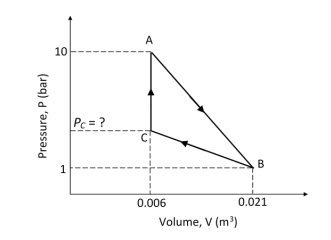
\includegraphics[width=0.6\columnwidth]{q20_thermo_2018.png} \caption*{} \label{fig:q20_thermo_2018} \end{figure}
    \hfill{\brak{\text{GATE XE 2018}}}

    \item One kmol of an ideal gas at 300 K and 10 bar is reversibly heated in a constant volume process to 500 K. It is then reversibly and isothermally expanded to 2 bar. Take $C_v = 20.8$ kJ/kmol.K and $R = 8.314$ kJ/kmol.K. The total heat supplied (in kJ) to the gas (up to 1 decimal place) is \underline{\hspace{2cm}}.
    \hfill{\brak{\text{GATE XE 2018}}}

    \item A rigid container is completely filled with a liquid having a constant isothermal compressibility of $1.09 \times 10^{-4}$ bar$^{-1}$ and a constant coefficient of volume expansion of $1.12 \times 10^{-3}$ K$^{-1}$. The liquid is initially at 300 K and 1 bar. Heat is supplied to the liquid to raise its temperature to 350 K. Assuming that no phase change occurs, the final pressure (in bar) of the liquid (up to 1 decimal place) is \underline{\hspace{2cm}}.
    \hfill{\brak{\text{GATE XE 2018}}}
\end{enumerate}
\clearpage

\section*{F : POLYMER SCIENCE AND ENGINEERING}
\begin{enumerate}
    \item Which one of the following polymers occurs naturally?
    \hfill{\brak{\text{GATE XE 2018}}}
    \begin{enumerate}[label=\Alph*)]
        \begin{multicols}{4}
            \item Bakelite
            \item Teflon
            \item Cellulose
            \item Perspex
        \end{multicols}
    \end{enumerate}

    \item The order of average molecular weights of a polymer is
    \hfill{\brak{\text{GATE XE 2018}}}
    \begin{enumerate}[label=\Alph*)]
        \item $M_z > M_w > M_v > M_n$
        \item $M_w > M_z > M_n > M_v$
        \item $M_n > M_w > M_v > M_z$
        \item $M_z > M_v > M_n > M_w$
    \end{enumerate}

    \item Rubbers are a class of polymer known for
    \hfill{\brak{\text{GATE XE 2018}}}
    \begin{enumerate}[label=\Alph*)]
        \item High intermolecular forces
        \item High $T_g$ polymers
        \item Crystalline polymers
        \item Low intermolecular forces
    \end{enumerate}

    \item Nylon 6 is manufactured from
    \hfill{\brak{\text{GATE XE 2018}}}
    \begin{enumerate}[label=\Alph*)]
        \item Sebacic acid and hexamethylene diamine
        \item Caprolactam
        \item Adipic acid and hexamethylene diamine
        \item Caprolactone
    \end{enumerate}

    \item Storage modulus and tan $\delta$ of a polymer are experimentally measured by
    \hfill{\brak{\text{GATE XE 2018}}}
    \begin{enumerate}[label=\Alph*)]
        \item Differential scanning calorimetry
        \item Thermogravimetric analysis
        \item Thermomechanical analysis
        \item Dynamic mechanical thermal analysis
    \end{enumerate}

    \item A plastic bucket is manufactured by
    \hfill{\brak{\text{GATE XE 2018}}}
    \begin{enumerate}[label=\Alph*)]
        \item Compression moulding
        \item Injection moulding
        \item Extrusion
        \item Blow moulding
    \end{enumerate}

    \item The monomers, A and B with reactivity ratios $r_A$ and $r_B$, form alternate copolymers when,
    \hfill{\brak{\text{GATE XE 2018}}}
    \begin{enumerate}[label=\Alph*)]
        \begin{multicols}{4}
            \item $r_A = r_B = 0$
            \item $r_A = r_B = 1$
            \item $r_A > 1, r_B > 1$
            \item $r_A < 1, r_B < 1$
        \end{multicols}
    \end{enumerate}

    \item The degree of polymerization of a poly(methyl methacrylate) sample having number average molecular weight of 1,50,000 g/mol is \underline{\hspace{2cm}}.
    (C = 12, H = 1, O = 16 g/mol).
    \hfill{\brak{\text{GATE XE 2018}}}

    \item If the heat of fusion of 100 \% crystalline polyethylene is 290 mJ/mg, a sample of polyethylene with heat of fusion of 141 mJ/mg will have \underline{\hspace{2cm}} \% crystallinity.
    \hfill{\brak{\text{GATE XE 2018}}}

    \item Match the following:
    \begin{table}[h!] \centering \caption*{} \label{tab:q10_poly_2018}
        \begin{tabular}{|l|l|} \hline
        P. Butyl rubber & 1. Metallocene polymerization \\
        Q. Cold SBR & 2. Cationic polymerization \\
        R. Poly(ethylene terephthalate) & 3. Redox polymerization \\
        S. Polypropylene & 4. Condensation polymerization \\ \hline
        \end{tabular}
    \end{table}
    \hfill{\brak{\text{GATE XE 2018}}}
    \begin{enumerate}[label=\Alph*)]
        \begin{multicols}{2}
            \item P-3; Q-1; R-2; S-1
            \item P-2; Q-3; R-1; S-4
            \item P-4; Q-3; R-1; S-2
            \item P-2; Q-3; R-4; S-1
        \end{multicols}
    \end{enumerate}

    \item Match the following:
    \begin{table}[h!] \centering \caption*{} \label{tab:q11_poly_2018}
        \begin{tabular}{|l|l|} \hline
        P. Polyaramid & 1. Baby-feeding nipple \\
        Q. Polytetrafluoroethylene & 2. Optical glasses \\
        R. Polycarbonate & 3. Non-stick cookware \\
        S. Poly(dimethyl siloxane) & 4. Bullet-proof jacket \\ \hline
        \end{tabular}
    \end{table}
    \hfill{\brak{\text{GATE XE 2018}}}
    \begin{enumerate}[label=\Alph*)]
        \begin{multicols}{2}
            \item P-4; Q-3; R-2; S-1
            \item P-2; Q-3; R-4; S-1
            \item P-4; Q-1; R-2; S-3
            \item P-3; Q-4; R-2; S-1
        \end{multicols}
    \end{enumerate}

    \item Flexible PVC tubes are used for watering. If some organic solvents are passed through this tube, it becomes stiff. This is due to the fact that the organic solvents
    \hfill{\brak{\text{GATE XE 2018}}}
    \begin{enumerate}[label=\Alph*)]
        \item plasticize PVC and raise $T_g$.
        \item remove plasticizer and raise $T_g$.
        \item remove plasticizer and lower $T_g$.
        \item react with PVC and increase $T_g$.
    \end{enumerate}

    \item Match the following:
    \begin{table}[h!] \centering \caption*{} \label{tab:q13_poly_2018}
        \begin{tabular}{|l|l|} \hline
        P. Plastic egg container & 1. Injection moulding \\
        Q. Water tank & 2. Extrusion \\
        R. Chair & 3. Rotational moulding \\
        S. Cable & 4. Thermoforming \\ \hline
        \end{tabular}
    \end{table}
    \hfill{\brak{\text{GATE XE 2018}}}
    \begin{enumerate}[label=\Alph*)]
        \begin{multicols}{2}
            \item P-3; Q-1; R-4; S-2
            \item P-4; Q-3; R-2; S-1
            \item P-2; Q-3; R-4; S-1
            \item P-4; Q-3; R-1; S-2
        \end{multicols}
    \end{enumerate}

    \item Match the following:
    \begin{table}[h!] \centering \caption*{} \label{tab:q14_poly_2018}
        \begin{tabular}{|l|l|} \hline
        P. Flame retardant & 1. 4-Methyl-2,6-di-t-butyl phenol \\
        Q. UV absorber & 2. Azocarbonamide \\
        R. Blowing agent & 3. Phenyl salisylate \\
        S. Antioxidant & 4. Aluminium trihydrate \\ \hline
        \end{tabular}
    \end{table}
    \hfill{\brak{\text{GATE XE 2018}}}
    \begin{enumerate}[label=\Alph*)]
        \begin{multicols}{2}
            \item P-4; Q-1; R-2; S-3
            \item P-4; Q-3; R-2; S-1
            \item P-3; Q-4; R-2; S-1
            \item P-2; Q-4; R-1; S-3
        \end{multicols}
    \end{enumerate}

    \item A plot of strain (\%) versus time of a polymer is given below. Based on this plot and the properties as mentioned below, find out the correct combination.
    \begin{figure}[H] \centering 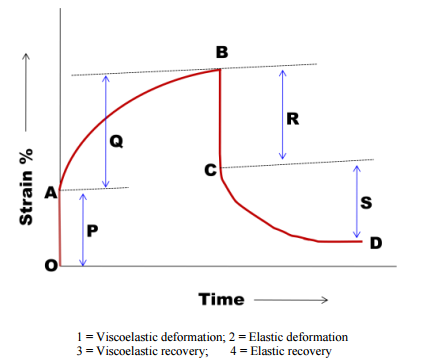
\includegraphics[width=0.7\columnwidth]{q15_poly_2018.png} \caption*{} \label{fig:q15_poly_2018} \end{figure}
    1 = Viscoelastic deformation; 2 = Elastic deformation \\
    3 = Viscoelastic recovery; 4 = Elastic recovery
    \hfill{\brak{\text{GATE XE 2018}}}
    \begin{enumerate}[label=\Alph*)]
        \begin{multicols}{2}
            \item P-1; Q-4; R-2; S-3
            \item P-2; Q-3; R-4; S-1
            \item P-3; Q-1; R-2; S-4
            \item P-2; Q-1; R-4; S-3
        \end{multicols}
    \end{enumerate}

    \item The plot shows apparent viscosity versus shear rate of Newtonian, Dilatent and Pseudoplastic fluids. Based on this plot and the fluid behaviour as mentioned below, find out the correct combination.
    \begin{figure}[H] \centering 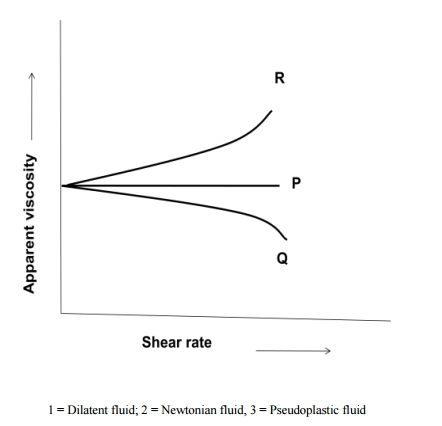
\includegraphics[width=0.6\columnwidth]{q16_poly_2018.png} \caption*{} \label{fig:q16_poly_2018} \end{figure}
    \hfill{\brak{\text{GATE XE 2018}}}
    \begin{enumerate}[label=\Alph*)]
        \begin{multicols}{2}
            \item P-1; Q-2; R-3
            \item P-3; Q-1; R-2
            \item P-2; Q-3; R-1
            \item P-2; Q-3; Q-1
        \end{multicols}
    \end{enumerate}

    \item Plot of the modulus versus temperature of different types of polymers is given below. Based on this plot and the nature of the polymers as mentioned below, find out the correct combination.
    \begin{figure}[H] \centering 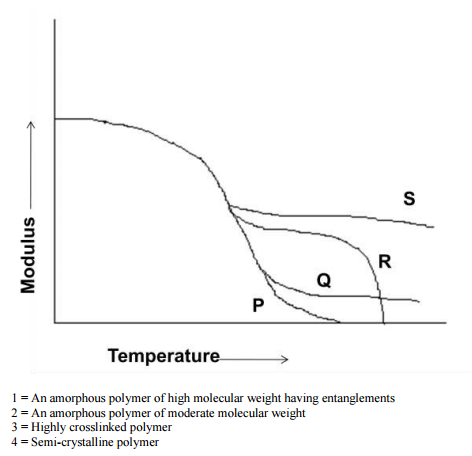
\includegraphics[width=0.7\columnwidth]{q17_poly_2018.png} \caption*{} \label{fig:q17_poly_2018} \end{figure}
    \hfill{\brak{\text{GATE XE 2018}}}
    \begin{enumerate}[label=\Alph*)]
        \begin{multicols}{2}
            \item P-2; Q-1; R-3; S-4
            \item P-1; Q-2; R-3; S-4
            \item P-2; Q-1; R-4; S-3
            \item P-1; Q-3; R-4; S-2
        \end{multicols}
    \end{enumerate}

    \item The $T_g$ of homopolymers of A and B are +100 $\degree$C and -70 $\degree$C respectively. The $T_g$ of a random copolymer of A and B having 40 wt\% A and 60 wt\% B is \underline{\hspace{2cm}} $\degree$C.
    \hfill{\brak{\text{GATE XE 2018}}}

    \item The number average molecular weight of a polymer prepared from HO(CH$_2$)$_{14}$COOH is 24,000 g/mol. The conversion of the monomer required to reach the above molecular weight is \underline{\hspace{2cm}} \%. (C = 12, H = 1, O = 16 g/mol).
    \hfill{\brak{\text{GATE XE 2018}}}

    \item Glass fibers in nylon provide reinforcement. The modulus of elasticity for each component of the composite is; $E_{glass} = 10.5 \times 10^6$ psi; $E_{nylon} = 0.4 \times 10^6$ psi. If the nylon contains 30 vol \% E-glass, the fraction of the applied force is carried by the glass fiber is \underline{\hspace{2cm}}. (Assume that both glass fiber and nylon have equal strain).
    \hfill{\brak{\text{GATE XE 2018}}}

    \item The solubility parameter of a polymer having cohesive energy density ($E_{coh}$) 43870 J/mol and molar volume (V) 136 cm$^3$/mol is \underline{\hspace{2cm}} (J/cm$^3$)$^{1/2}$.
    \hfill{\brak{\text{GATE XE 2018}}}

    \item The heat of polymerization of styrene is 20 Kcal/mol. Heat of $5 \times 10^5$ Kcal will be released on polymerization of \underline{\hspace{2cm}} Kg of styrene (C = 12 and H = 1 g/mol).
    \hfill{\brak{\text{GATE XE 2018}}}
\end{enumerate}
\clearpage

\section*{G: FOOD TECHNOLOGY}
\begin{enumerate}
    \item Which of the following is oil soluble pigment present in fruits and vegetables?
    \hfill{\brak{\text{GATE XE 2018}}}
    \begin{enumerate}[label=\Alph*)]
        \begin{multicols}{4}
            \item Flavonoids
            \item Carotenoids
            \item Anthocyanins
            \item Tannins
        \end{multicols}
    \end{enumerate}

    \item Which of the following represent the group of saturated fatty acids?
    \hfill{\brak{\text{GATE XE 2018}}}
    \begin{enumerate}[label=\Alph*)]
        \begin{multicols}{2}
            \item Lauric, Myristic, Arachidic
            \item Palmitic, Linoleic, Linolenic
            \item Capric, Stearic \& Oleic
            \item Behenic, Caprylic, Arachidonic
        \end{multicols}
    \end{enumerate}

    \item The anti-nutritional factor present in fava bean is
    \hfill{\brak{\text{GATE XE 2018}}}
    \begin{enumerate}[label=\Alph*)]
        \begin{multicols}{2}
            \item Gossypol
            \item Curcine
            \item Vicine
            \item Cyanogen
        \end{multicols}
    \end{enumerate}

    \item Irradiation carried out to reduce viable non-spore forming pathogenic bacteria using a dose between 3 to 10 kGy is called
    \hfill{\brak{\text{GATE XE 2018}}}
    \begin{enumerate}[label=\Alph*)]
        \begin{multicols}{2}
            \item Radurization
            \item Thermoradiation
            \item Radappertization
            \item Radicidation
        \end{multicols}
    \end{enumerate}

    \item Identify the correct statement related to the viscosity of Newtonian fluids from the following
    \hfill{\brak{\text{GATE XE 2018}}}
    \begin{enumerate}[label=\Alph*)]
        \item It is not influenced by temperature
        \item It increases with shearing rate
        \item It decreases with shearing rate
        \item It is not influenced by shearing rate
    \end{enumerate}

    \item Adult male Wistar rats were fed with a protein based diet. Total 150 g of protein was ingested per animal. If the average weight increased from 110 g to 350 g after the end of the experiment, the Protein efficiency ratio of the given protein would be \underline{\hspace{2cm}} (up to two decimal points).
    \hfill{\brak{\text{GATE XE 2018}}}

    \item The initial moisture content of a food on wet basis is 50.76\%. Its moisture content (\%) on dry basis is \underline{\hspace{2cm}}. (up to two decimal points).
    \hfill{\brak{\text{GATE XE 2018}}}

    \item The oxygen transmission rate through a 2.54 x 10$^{-3}$ cm thick low density polyethylene film with air on one side and inert gas on the other side is $3.5 \times 10^{-6}$ mL cm$^{-2}$ s$^{-1}$. Oxygen partial pressure difference across the film is 0.21 atm. The permeability coefficient of the film to oxygen is \underline{\hspace{2cm}} x 10$^{-11}$ mL (STP) cm cm$^{-2}$ s$^{-1}$ (cm Hg)$^{-1}$.
    \hfill{\brak{\text{GATE XE 2018}}}

    \item Ambient air at 30$^{\circ}$C dry bulb temperature and 80\% relative humidity was heated to a dry bulb temperature of 80$^{\circ}$C in a heat exchanger by indirect heating. The amount of moisture gain (g kg$^{-1}$ dry air) during the process would be \underline{\hspace{2cm}}.
    \hfill{\brak{\text{GATE XE 2018}}}

    \item Match the commodity in Group I with the bioactive constituent in Group II
    \begin{table}[h!] \centering \caption*{} \label{tab:q10_food_2018}
        \begin{tabular}{ll}
            \textbf{Group I} & \textbf{Group II} \\
            P. Ginger & 1. Lutein \\
            Q. Green tea & 2. Gingerol \\
            R. Spinach & 3. Curcumin \\
            S. Turmeric & 4. Epigallocatechin gallate
        \end{tabular}
    \end{table}
    \hfill{\brak{\text{GATE XE 2018}}}
    \begin{enumerate}[label=\Alph*)]
        \item P-1, Q-2, R-3, S-4
        \item P-2, Q-4, R-1, S-3
        \item P-4, Q-1, R-3, S-2
        \item P-2, Q-3, R-1, S-4
    \end{enumerate}

    \item Match the process operation in Group I with the separated constituent in Group II
    \begin{table}[h!] \centering \caption*{} \label{tab:q11_food_2018}
        \begin{tabular}{ll}
            \textbf{Group I} & \textbf{Group II} \\
            P. Extraction & 1. Phospholipids \\
            Q. Degumming & 2. Free fatty acids \\
            R. Neutralization & 3. Pigments \\
            S. Bleaching & 4. Crude oil
        \end{tabular}
    \end{table}
    \hfill{\brak{\text{GATE XE 2018}}}
    \begin{enumerate}[label=\Alph*)]
        \item P-3, Q-2, R-4, S-1
        \item P-4, Q-3, R-1, S-2
        \item P-4, Q-1, R-2, S-3
        \item P-4, Q-1, R-3, S-2
    \end{enumerate}

    \item Match the spoilage symptom in Group I with the causative microorganism in Group II
    \begin{table}[h!] \centering \caption*{} \label{tab:q12_food_2018}
        \begin{tabular}{ll}
            \textbf{Group I} & \textbf{Group II} \\
            P. Green rot of eggs & 1. Micrococcus spp. \\
            Q. Putrid swell in canned fish & 2. Serratia marcescens \\
            R. Red bread & 3. Pseudomonas fluorescens \\
            S. Yellow discoloration of meat & 4. Clostridium sporogenes
        \end{tabular}
    \end{table}
    \hfill{\brak{\text{GATE XE 2018}}}
    \begin{enumerate}[label=\Alph*)]
        \item P-4, Q-3, R-2, S-1
        \item P-2, Q-1, R-4, S-3
        \item P-3, Q-4, R-2, S-1
        \item P-1, Q-4, R-3, S-2
    \end{enumerate}

    \item Match the fermented product in Group I with the base material in Group II
    \begin{table}[h!] \centering \caption*{} \label{tab:q13_food_2018}
        \begin{tabular}{ll}
            \textbf{Group I} & \textbf{Group II} \\
            P. Sake & 1. Milk \\
            Q. Chhurpi & 2. Cabbage \\
            R. Natto & 3. Rice \\
            S. Sauerkraut & 4. Soybean
        \end{tabular}
    \end{table}
    \hfill{\brak{\text{GATE XE 2018}}}
    \begin{enumerate}[label=\Alph*)]
        \item P-3, Q-1, R-4, S-2
        \item P-1, Q-3, R-4, S-2
        \item P-4, Q-1, R-3, S-2
        \item P-3, Q-2, R-1, S-4
    \end{enumerate}

    \item Match the operation in Group I with the process in Group II
    \begin{table}[h!] \centering \caption*{} \label{tab:q14_food_2018}
        \begin{tabular}{ll}
            \textbf{Group I} & \textbf{Group II} \\
            P. Cleaning & 1. Quality separation \\
            Q. Grading & 2. Clarification \\
            R. Size reduction & 3. Screening \\
            S. Filtration & 4. Comminution
        \end{tabular}
    \end{table}
    \hfill{\brak{\text{GATE XE 2018}}}
    \begin{enumerate}[label=\Alph*)]
        \item P-1, Q-3, R-4, S-2
        \item P-4, Q-1, R-3, S-2
        \item P-2, Q-4, R-1, S-3
        \item P-3, Q-1, R-4, S-2
    \end{enumerate}

    \item Out of 7 principles of HACCP system, 4 are listed below. Arrange these principles in the order in which they are applied.
    (P) Conduct a hazard analysis
    (Q) Establish monitoring process
    (R) Establish critical limit
    (S) Establish record keeping and documentation process
    \hfill{\brak{\text{GATE XE 2018}}}
    \begin{enumerate}[label=\Alph*)]
        \begin{multicols}{4}
            \item P, R, Q, S
            \item Q, R, P, S
            \item P, Q, R, S
            \item R, S, P, Q
        \end{multicols}
    \end{enumerate}

    \item Apple juice of 10\% total solids (TS) is being concentrated in a single effect evaporator working with a surface condenser to 40\% TS under a vacuum of 20 kPa. After some time the vacuum pump stops but the evaporation process continued. Choose the combination of possible implications from the following.
    (P) Product quality is affected
    (Q) Substantial increase in thermal energy requirement
    (R) Decrease in the rate of evaporation
    \hfill{\brak{\text{GATE XE 2018}}}
    \begin{enumerate}[label=\Alph*)]
        \begin{multicols}{4}
            \item P \& Q
            \item Q \& R
            \item R \& P
            \item P, Q \& R
        \end{multicols}
    \end{enumerate}

    \item Identify an example of a classical diffusional mass transfer process without involving heat, among the following.
    \hfill{\brak{\text{GATE XE 2018}}}
    \begin{enumerate}[label=\Alph*)]
        \item Drying of food grains
        \item Carbonation of beverages
        \item Distillation of alcohol
        \item Concentration of fruit juice
    \end{enumerate}

    \item For an enzyme catalyzed reaction S$\rightarrow$P, the kinetic parameters are:
    [S] = 40 $\mu$M, V$_o$ = 9.6 $\mu$M s$^{-1}$ and V$_{max}$ = 12.0 $\mu$M s$^{-1}$.
    The K$_m$ of the enzyme in $\mu$M will be \underline{\hspace{2cm}} (up to one decimal points).
    \hfill{\brak{\text{GATE XE 2018}}}

    \item A microbial sample taken at 10 AM contained $1 \times 10^5$ CFU/mL. The count reached to $1 \times 10^{10}$ CFU/mL at 8 PM of the same day. The growth rate (h$^{-1}$) of the microorganism would be \underline{\hspace{2cm}} (up to two decimal points).
    \hfill{\brak{\text{GATE XE 2018}}}

    \item Black pepper is ground from an equivalent particle size of 6 mm to 0.12 mm using a 10 hp motor. Assuming Rittinger's equation and that 1 hp = 745.7 W, the power (hp) of motor required to fine grind black pepper to 0.08 mm would be \underline{\hspace{2cm}} (up to two decimal points).
    \hfill{\brak{\text{GATE XE 2018}}}

    \item Green pea (average diameter 0.8 cm) is frozen in a blast freezer operating at -40$^{\circ}$C and with a surface heat transfer coefficient of 30 W m$^{-2}$ K$^{-1}$. The thermal conductivity of pea is 2.5 W m$^{-1}$K$^{-1}$, and latent heat of crystallization is $2.74 \times 10^2$ kJ kg$^{-1}$. If the freezing point of pea is -1$^{\circ}$C and the density is 1160 kg m$^{-3}$, the freezing time in minutes will be \underline{\hspace{2cm}} (up to two decimal points).
    \hfill{\brak{\text{GATE XE 2018}}}

    \item The rate of heat transfer from a metal plate is 1000 W m$^{-2}$. The surface temperature of the plate is 120$^{\circ}$C and ambient temperature is 20$^{\circ}$C. The convective heat transfer coefficient (W m$^{-2}$ $^{\circ}$C$^{-1}$) using the Newton's law of cooling will be \underline{\hspace{2cm}}.
    \hfill{\brak{\text{GATE XE 2018}}}
\end{enumerate}
\clearpage

\section*{H: ATMOSPHERIC AND OCEANIC SCIENCES}
\begin{enumerate}
    \item The most abundant gas in the atmosphere among inert gases is
    \hfill{\brak{\text{GATE XE 2018}}}
    \begin{enumerate}[label=\Alph*)]
        \begin{multicols}{4}
            \item Helium
            \item Argon
            \item Neon
            \item Krypton
        \end{multicols}
    \end{enumerate}

    \item The pair of variables that always exhibit monotonic decrease with height in the atmosphere is
    \hfill{\brak{\text{GATE XE 2018}}}
    \begin{enumerate}[label=\Alph*)]
        \begin{multicols}{2}
            \item Pressure, Temperature
            \item Pressure, Ozone concentration
            \item Air Density, Pressure
            \item Temperature, Water Vapour
        \end{multicols}
    \end{enumerate}

    \item Correct order of the maximum vertical extent of atmospheric circulation cells is
    \hfill{\brak{\text{GATE XE 2018}}}
    \begin{enumerate}[label=\Alph*)]
        \begin{multicols}{2}
            \item Hadley > Ferrel > Polar
            \item Polar > Hadley > Ferrel
            \item Hadley > Polar > Ferrel
            \item Ferrel > Hadley > Polar
        \end{multicols}
    \end{enumerate}

    \item Analysis of an atmospheric variable shows prominent modes at 5, 40 and 1460 days. These modes correspond respectively to
    \hfill{\brak{\text{GATE XE 2018}}}
    \begin{enumerate}[label=\Alph*)]
        \begin{multicols}{2}
            \item Tidal, MJO and ENSO
            \item Synoptic, MJO and ENSO
            \item Synoptic, MJO and Decadal
            \item Tidal, Milankhovich and ENSO
        \end{multicols}
    \end{enumerate}

    \item Atmospheric vertical profile of temperature is measured by radiosonde. Equivalent instruments for measuring ocean temperature profile among the following are:
    (P) drifting buoy (Q) ARGO float (R) current mooring (S) XBT
    \hfill{\brak{\text{GATE XE 2018}}}
    \begin{enumerate}[label=\Alph*)]
        \begin{multicols}{4}
            \item Q, R, S
            \item Q, S
            \item R, S
            \item P, R, S
        \end{multicols}
    \end{enumerate}

    \item When deep water sinks in the North Atlantic and moves away from where it formed, it gets
    \hfill{\brak{\text{GATE XE 2018}}}
    \begin{enumerate}[label=\Alph*)]
        \item richer in oxygen and nutrients
        \item less acidic and richer in metals
        \item richer in CO$_2$ and poorer in O$_2$
        \item richer in CO$_2$ and O$_2$
    \end{enumerate}

    \item The speed of sound in the ocean depends on
    \hfill{\brak{\text{GATE XE 2018}}}
    \begin{enumerate}[label=\Alph*)]
        \item temperature alone
        \item temperature and pressure
        \item temperature and salinity
        \item temperature, salinity and pressure
    \end{enumerate}

    \item In a numerical weather prediction model with a horizontal grid resolution of 50 km, convective cloud processes are parameterized, because
    \hfill{\brak{\text{GATE XE 2018}}}
    \begin{enumerate}[label=\Alph*)]
        \item Cloud physics is not known for modelling
        \item Models cannot handle phase change
        \item Cloud size is larger than the grid size
        \item Cloud size is much smaller than the grid size
    \end{enumerate}

    \item Figure below shows SST anomaly (in $^{\circ}$C). It is associated with the phenomenon known as
    \begin{figure}[H] \centering 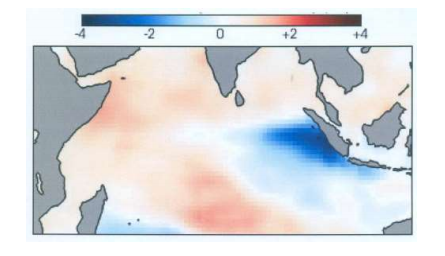
\includegraphics[width=0.7\columnwidth]{q9_atmos_2018.png} \caption*{} \label{fig:q9_atmos_2018} \end{figure}
    \hfill{\brak{\text{GATE XE 2018}}}
    \begin{enumerate}[label=\Alph*)]
        \begin{multicols}{2}
            \item El Nino
            \item Indian Ocean dipole
            \item La Nina
            \item MJO
        \end{multicols}
    \end{enumerate}

    \item For an inviscid and barotropic ocean of constant depth (D), a water parcel with initial vorticity 2$\Omega$ is displaced from the equator to the north pole. Latitudinal variation of the parcel vorticity ($\zeta$) is well represented by the curve
    \begin{figure}[H] \centering 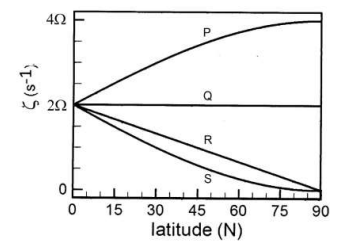
\includegraphics[width=0.6\columnwidth]{q10_atmos_2018.png} \caption*{} \label{fig:q10_atmos_2018} \end{figure}
    \hfill{\brak{\text{GATE XE 2018}}}
    \begin{enumerate}[label=\Alph*)]
        \begin{multicols}{4}
            \item S
            \item Q
            \item P
            \item R
        \end{multicols}
    \end{enumerate}

    \item A wave progresses up an estuary of decreasing water depth. If friction is neglected, then
    \hfill{\brak{\text{GATE XE 2018}}}
    \begin{enumerate}[label=\Alph*)]
        \item wave amplitude decreases and wave length increases
        \item wave amplitude increases and wave length decreases
        \item wave amplitude decreases and wave length decreases
        \item wave amplitude increases and wave length increases
    \end{enumerate}

    \item In the Ekman flow limit, directions of ocean surface current and the geostrophic wind are
    \hfill{\brak{\text{GATE XE 2018}}}
    \begin{enumerate}[label=\Alph*)]
        \item the same
        \item surface current is 45$^{\circ}$ to the left of the geostrophic wind
        \item surface current is 45$^{\circ}$ to the right of the geostrophic wind
        \item exactly opposite to each other
    \end{enumerate}

    \item 
    \begin{figure}[H] \centering 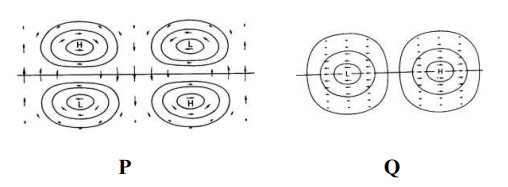
\includegraphics[width=\columnwidth]{q13_atmos_2018.png} \caption*{} \label{fig:q13_atmos_2018} \end{figure}
    P and Q respectively describe flow fields corresponding to
    \hfill{\brak{\text{GATE XE 2018}}}
    \begin{enumerate}[label=\Alph*)]
        \item Mid latitude Rossby and Polar gravity waves
        \item Equatorial Rossby and Equatorial Kelvin waves
        \item Midlatitude gravity and Polar Rossby waves
        \item Equatorial Kelvin and Equatorial Rossby waves
    \end{enumerate}

    \item On the summer solstice day, the maximum incident shortwave radiation at the top of the atmosphere over the equator (up to one decimal place) is \underline{\hspace{2cm}} W m$^{-2}$. (Take solar constant as 1368 W m$^{-2}$).
    \hfill{\brak{\text{GATE XE 2018}}}

    \item In an isothermal atmosphere having a temperature of 15$^{\circ}$C, the height at which pressure decreases to 1/10 of its value at the surface is \underline{\hspace{2cm}} km. (Give the answer to two decimal places.) Take g = 9.8 m s$^{-2}$, gas constant R = 287 J kg$^{-1}$ K$^{-1}$.
    \hfill{\brak{\text{GATE XE 2018}}}

    \item At 30$^{\circ}$N and 700 hPa pressure level, wind field is in gradient balance. If the gradient wind speed is 50 m s$^{-1}$ and radius of curvature of the flow is 50 km, the corresponding geostrophic wind speed is \underline{\hspace{2cm}} m s$^{-1}$. (Give the answer to one decimal place.) Take the angular velocity of the Earth as $7.3 \times 10^{-5}$ s$^{-1}$.
    \hfill{\brak{\text{GATE XE 2018}}}

    \item In a tropical cyclone over the Pacific Ocean, surface pressure at 500 km from the cyclone centre is 1000 hPa. Surface pressure at the centre is 900 hPa. Sea surface temperature and surface air temperature remain constant at 28$^{\circ}$C and 27$^{\circ}$C, respectively. Difference in potential temperature between 500 km and cyclone centre is \underline{\hspace{2cm}} K. (Give the answer to two decimal places.) Take g = 9.8 m s$^{-2}$, $C_p$ = 1005 J kg$^{-1}$ K$^{-1}$, gas constant R = 287 J kg$^{-1}$ K$^{-1}$.
    \hfill{\brak{\text{GATE XE 2018}}}

    \item A cloud forms by the lifting of moist air from the surface with the initial conditions $T_0$ = 30$^{\circ}$C, RH = 80\% and $P_0$ = 1005 hPa. If the vapour pressure of this parcel at 500 hPa is 6.5 hPa, the liquid water content of the parcel if no precipitation takes place is \underline{\hspace{2cm}} gm kg$^{-1}$. (Give the answer to one decimal place.) Saturation vapour pressure of water at 30$^{\circ}$C is 42.43 hPa.
    \hfill{\brak{\text{GATE XE 2018}}}

    \item A numerical model of the atmosphere uses sigma ($\sigma$) coordinate system in vertical. At locations P and Q, surface pressures are 1005 hPa and 500 hPa, respectively. Absolute difference in the heights of $\sigma$ = 0.9 level between these locations is \underline{\hspace{2cm}} meters. (Give the answer to one decimal place.) Layer mean temperatures at P and Q are 300 K and 270 K, respectively. (Take g = 9.8 m s$^{-2}$ gas constant R = 287 J kg$^{-1}$ K$^{-1}$).
    \hfill{\brak{\text{GATE XE 2018}}}

    \item If difference in sea surface elevation is 1 m in 100 km at 30$^{\circ}$ N latitude, the corresponding geostrophic current is \underline{\hspace{2cm}} m s$^{-1}$. (Give the answer to one decimal place.) Take g = 9.8 m s$^{-2}$ and angular velocity of the Earth = $7.3 \times 10^{-5}$ s$^{-1}$.
    \hfill{\brak{\text{GATE XE 2018}}}

    \item If wind speed over ocean surface is 10 m s$^{-1}$, air-sea interface momentum flux is \underline{\hspace{2cm}} N m$^{-2}$. (Give the answer to two decimal places.) Surface air temperature and pressure are 27$^{\circ}$C and 1000 hPa, respectively. Take drag coefficient as 0.001 and gas constant R = 287 J kg$^{-1}$ K$^{-1}$.
    \hfill{\brak{\text{GATE XE 2018}}}

    \item Let $L_x, L_y$ be length scales in x- and y-directions and corresponding mass transports are $M_x$ and $M_y$. The ratio of $M_x$ and $M_y$ (to nearest integer) is \underline{\hspace{2cm}}, if the ratio of $L_x$ and $L_y$ is 10 and vertical velocity is zero.
    \hfill{\brak{\text{GATE XE 2018}}}
\end{enumerate}

\end{document}